Le projet est pré-déployé sur la machine virtuelle (VM) fournie. Voici les étapes réalisées :

\begin{enumerate}
	\item Placer le code source du site web dans le répertoire suivant :
	\begin{itemize}[label=$\bullet$]
		\item \url{C:\wamp64\www\NomDuProjet}
	\end{itemize}
	\textit{NomDuProjet} est dans notre exemple : HanutA\_PrjDevWeb2324
	
	
	\item Créer le virtual host sur Wamp64 : dans ce cas, le lien vers le projet sera : \\ \url{http://prj2324.local}
	\begin{figure}[h]
		\centering
		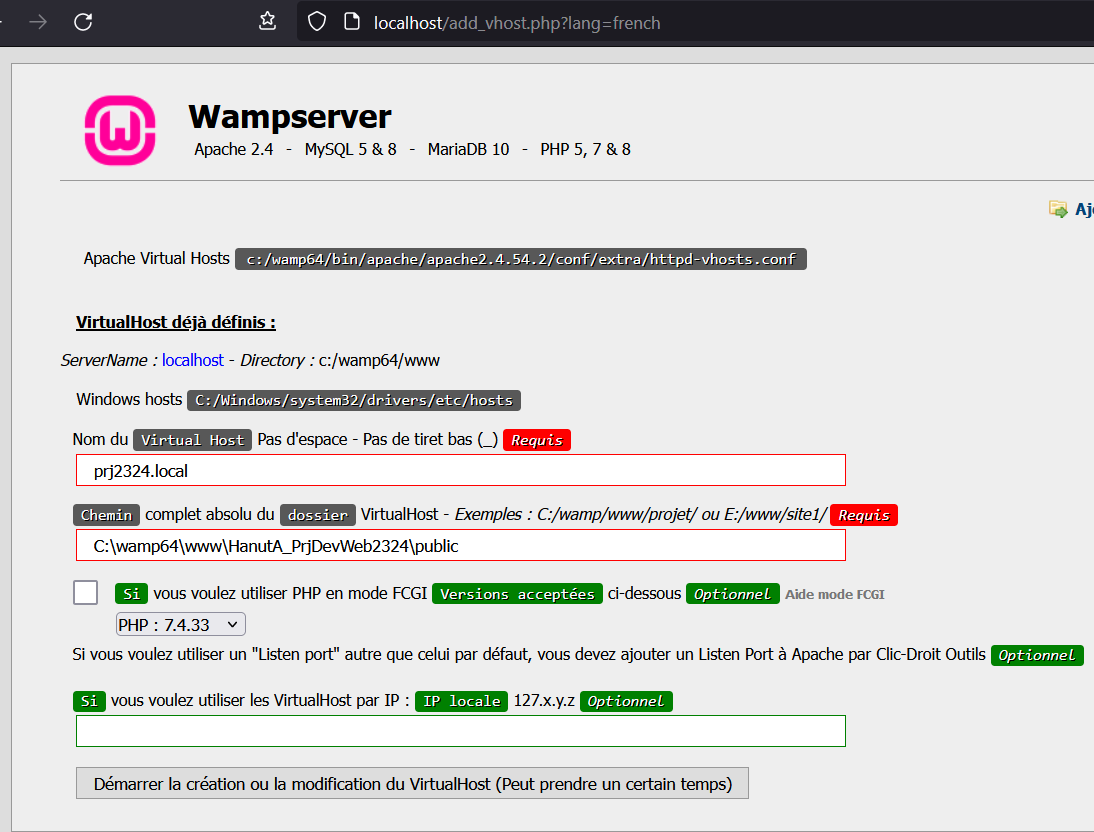
\includegraphics[keepaspectratio,width=15cm]{images/VirtualHost}
		\caption{Interface de création d'un VirtualHost via Wamp64}
	\end{figure}
\end{enumerate}